\documentclass[11pt,a4paper]{article}

\usepackage[utf8]{inputenc}
\usepackage[T1]{fontenc}
\usepackage{mathpazo}
\usepackage[scaled=0.92]{helvet}
\usepackage[margin=1in]{geometry}
\usepackage{graphicx}
\usepackage{amsmath,amssymb,amsfonts}
\usepackage{booktabs}
\usepackage{tabularx}
\usepackage{setspace}
\usepackage{titlesec}
\usepackage{fancyhdr}
\usepackage{float}
\usepackage{caption}
\usepackage{microtype}
\usepackage{tikz}
\usepackage{xcolor}
\usepackage{listings}
\usepackage[hidelinks]{hyperref}

\usetikzlibrary{shapes.geometric, arrows.meta, positioning, calc, matrix, fit, backgrounds}

\setstretch{1.15}
\setlength{\parindent}{0pt}
\setlength{\parskip}{0.8em}
\sloppy

\titleformat{\section}{\normalfont\large\bfseries\sffamily}{\thesection}{1em}{}
\titleformat{\subsection}{\normalfont\normalsize\bfseries\sffamily}{\thesubsection}{1em}{}
\titleformat{\subsubsection}{\normalfont\normalsize\itshape\sffamily}{\thesubsubsection}{1em}{}

\pagestyle{fancy}
\fancyhf{}
\fancyhead[L]{\small\sffamily Matriks untuk RPL}
\fancyhead[R]{\small\sffamily\thepage}
\renewcommand{\headrulewidth}{0.4pt}

\captionsetup{font=small,labelfont=bf,labelsep=period}

\renewenvironment{abstract}
{\small
	\begin{center}\textbf{\sffamily Abstrak}\end{center}
	\begin{quote}}
	{\end{quote}}

\lstdefinestyle{code}{
	basicstyle=\ttfamily\small,
	frame=single,
	rulecolor=\color{black},
	breaklines=true,
	showstringspaces=false,
	columns=fullflexible,
	keepspaces=true,
	framesep=6pt,
	aboveskip=1em,
	belowskip=1em,
	xleftmargin=0pt
}

\lstdefinestyle{out}{
	basicstyle=\ttfamily\small,
	frame=tb,
	rulecolor=\color{black},
	breaklines=true,
	showstringspaces=false,
	columns=fullflexible,
	keepspaces=true,
	framesep=4pt,
	aboveskip=1em,
	belowskip=1em
}

\title{\vspace{-1.5cm}\textbf{\sffamily\LARGE Matriks dan Operasi Matriks untuk Rekayasa Perangkat Lunak\\ Modul Belajar dengan Visual yang Dapat Dibaca Tanpa Melihat}}
\author{
	\textbf{Muhammad Riduwan Khafidi} \\
	\small Program Studi Teknik Rekayasa Perangkat Lunak \\
	\small Politeknik Negeri Batam \\
	\small \texttt{4342611034@students.polibatam.ac.id}
}
\date{\small\today}

\begin{document}

\maketitle
\thispagestyle{empty}

\begin{abstract}
	Modul ini mengajarkan matriks sebagai model matematis untuk data berstruktur baris-kolom dalam rekayasa perangkat lunak. Pembahasan mencakup definisi, anatomi, jenis-jenis, kesamaan, penjumlahan, pengurangan, perkalian skalar, perkalian matriks, determinan, dan invers. Setiap konsep dibuka dengan analogi konkret, dilengkapi contoh berangka yang ditulis langkah demi langkah, dan ditutup dengan tabel ringkas. Sepuluh visual dirancang hitam-putih dan disertai narasi pengganti gambar sehingga pembaca yang mengandalkan teks tetap dapat membayangkannya. Modul ini memuat tiga studi kasus berbeda: penilaian akademik otomatis, penyelesaian sistem persamaan linear, dan transformasi warna gambar digital. Setelah membaca modul ini, pembaca dapat memodelkan data berbentuk tabel menjadi matriks, melakukan operasi yang sah sesuai syarat dimensi, serta menyelesaikan sistem persamaan linear menggunakan invers.
\end{abstract}

\section{Pendahuluan}

\subsection{Analogi Pembuka: Lemari Laci Berlabel}

Bayangkan sebuah lemari arsip besar. Lemari ini punya beberapa baris laci. Setiap baris punya beberapa kolom laci. Setiap laci berlabel dua angka: nomor barisnya dan nomor kolomnya. Laci dengan label $(2,3)$ berarti laci yang berada di baris kedua, kolom ketiga.

Jika petugas ingin mengambil satu dokumen, ia cukup menyebut label laci. Jika petugas ingin memindahkan seluruh baris, ia cukup menyebut nomor barisnya. Jika petugas ingin menghitung total isi semua laci, ia menjumlahkan isi setiap laci yang beralamat sama dengan laci di lemari lain.

Matriks adalah lemari laci berlabel itu. Setiap elemen matriks punya alamat $(i,j)$ yang menyatakan baris dan kolom. Alamat itu membuat komputer dapat menyimpan data secara terstruktur, mengambil data secara cepat, dan melakukan operasi pada seluruh data sekaligus.

\subsection{Mengapa Topik Ini Penting}

Sistem akademik menyimpan nilai mahasiswa dalam bentuk tabel: baris untuk mahasiswa, kolom untuk mata kuliah. Sistem pengolahan citra menyimpan warna piksel dalam bentuk tabel: baris untuk posisi vertikal, kolom untuk posisi horizontal. Sistem navigasi menyimpan jarak antar kota dalam bentuk tabel: baris dan kolom untuk kota asal dan kota tujuan.

Semua tabel itu adalah matriks. Dengan matriks, operasi yang tadinya harus ditulis sebagai perulangan bersarang dapat dinyatakan sebagai satu operasi matematis. Penilaian akhir yang biasanya memerlukan lima baris kode perulangan dapat dinyatakan sebagai satu perkalian matriks dengan vektor bobot. Filter gambar yang biasanya memerlukan dua perulangan bersarang dapat dinyatakan sebagai satu penjumlahan matriks.

\subsection{Cara Membaca Modul Ini}

Setiap bagian mengikuti pola yang sama. Pertama, analogi konkret. Kedua, definisi formal. Ketiga, contoh berangka langkah demi langkah. Keempat, visual dengan narasi pengganti gambar. Kelima, tabel ringkas. Setiap konsep kunci diberi dua bagian tambahan: Cara Berpikir yang menjelaskan langkah mental menyelesaikan soal, dan Kalau Salah yang menunjukkan akibat jika langkah dilewati.

\subsection{Peta Pembahasan}

Bagian kedua membahas definisi dan anatomi matriks. Bagian ketiga membahas enam jenis matriks. Bagian keempat membahas kesamaan matriks. Bagian kelima membahas penjumlahan, pengurangan, dan perkalian skalar. Bagian keenam membahas perkalian matriks dengan matriks. Bagian ketujuh membahas determinan. Bagian kedelapan membahas invers. Bagian kesembilan memuat tiga studi kasus berturut-turut: nilai akademik, sistem persamaan linear, dan transformasi gambar. Bagian kesepuluh menyandingkan seluruh konsep. Bagian kesebelas dan keduabelas memberi daftar kesalahan umum dan lembar rujukan cepat.

\section{Definisi dan Anatomi Matriks}

\subsection{Analogi: Lemari Berlabel}

Lemari arsip punya baris dan kolom. Setiap laci diberi alamat dua angka: $(i,j)$. Matriks juga begitu. Setiap elemen $a_{ij}$ berada di baris $i$ dan kolom $j$. Angka $i$ disebut indeks baris. Angka $j$ disebut indeks kolom.

Jika kita menulis $a_{23}=80$, artinya elemen di baris kedua, kolom ketiga bernilai 80. Jika kita menulis $a_{32}=80$, artinya elemen di baris ketiga, kolom kedua bernilai 80. Kedua elemen itu berbeda alamat walaupun nilainya sama.

\subsection{Definisi Formal}

Matriks adalah susunan bilangan berbentuk persegi panjang yang disusun menurut baris dan kolom. Jika matriks $A$ memiliki $m$ baris dan $n$ kolom, maka ukurannya ditulis $m \times n$ dan disebut ordo atau dimensi. Elemen baris $i$ kolom $j$ ditulis $a_{ij}$. Notasi lengkapnya ditulis pada Persamaan~\ref{eq:matriks-umum} \cite{anton}.

\begin{equation}
	A_{m\times n}=\begin{bmatrix}
		a_{11} & a_{12} & \cdots & a_{1n} \\
		a_{21} & a_{22} & \cdots & a_{2n} \\
		\vdots & \vdots & \ddots & \vdots \\
		a_{m1} & a_{m2} & \cdots & a_{mn}
	\end{bmatrix}
	\label{eq:matriks-umum}
\end{equation}

Notasi singkatnya adalah $A=[a_{ij}]$ dengan $i=1,2,\ldots,m$ dan $j=1,2,\ldots,n$. Perhatikan anatomi matriks pada Gambar~\ref{fig:anatomi}.

\begin{figure}[H]
	\centering
	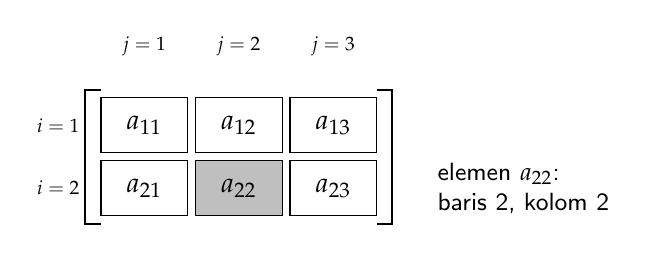
\begin{tikzpicture}[
			cell/.style={rectangle, draw=black, minimum width=1.1cm, minimum height=0.7cm, align=center, font=\sffamily},
			hl/.style={cell, fill=black!25},
			ilab/.style={font=\scriptsize\sffamily}
		]
		\node[ilab] at (0, 1.4) {$j=1$};
		\node[ilab] at (1.2, 1.4) {$j=2$};
		\node[ilab] at (2.4, 1.4) {$j=3$};

		\node[ilab, anchor=east] at (-0.7, 0.4) {$i=1$};
		\node[ilab, anchor=east] at (-0.7, -0.4) {$i=2$};

		\node[cell] at (0, 0.4) {$a_{11}$};
		\node[cell] at (1.2, 0.4) {$a_{12}$};
		\node[cell] at (2.4, 0.4) {$a_{13}$};
		\node[cell] at (0, -0.4) {$a_{21}$};
		\node[hl] at (1.2, -0.4) {$a_{22}$};
		\node[cell] at (2.4, -0.4) {$a_{23}$};

		\draw[thick] (-0.55, 0.85) -- (-0.75, 0.85) -- (-0.75, -0.85) -- (-0.55, -0.85);
		\draw[thick] (2.95, 0.85) -- (3.15, 0.85) -- (3.15, -0.85) -- (2.95, -0.85);

		\node[font=\small\sffamily, anchor=west, align=left] at (3.6, -0.4) {elemen $a_{22}$:\\baris 2, kolom 2};
	\end{tikzpicture}
	\caption{Anatomi matriks $2\times 3$ dengan penanda indeks baris $i$ dan indeks kolom $j$.}
	\label{fig:anatomi}
\end{figure}

Cara membaca Gambar~\ref{fig:anatomi}: gambar ini menampilkan kotak-kotak yang tersusun dua baris dan tiga kolom. Di atas setiap kolom ada label $j=1$, $j=2$, dan $j=3$. Di kiri setiap baris ada label $i=1$ dan $i=2$. Di dalam setiap kotak ada nama elemen dengan dua angka kecil: $a_{11}$, $a_{12}$, $a_{13}$ pada baris pertama, lalu $a_{21}$, $a_{22}$, $a_{23}$ pada baris kedua. Kotak $a_{22}$ diberi latar abu-abu dan di sebelah kanan ada keterangan "elemen $a_{22}$: baris 2, kolom 2". Inti pesan gambar ini adalah setiap elemen punya alamat dua angka, dan alamat itulah yang membedakan satu elemen dari yang lain.

\subsection{Hubungan dengan Pemrograman}

Matriks berhubungan langsung dengan tiga tipe data di pemrograman. Skalar berhubungan dengan variabel tunggal, misalnya \texttt{int~score~=~85}. Vektor berhubungan dengan array satu dimensi, misalnya \texttt{int[]~nilai~=~\{80,~85,~90\}}. Matriks berhubungan dengan array dua dimensi, misalnya \texttt{int[][]~M~=~\{\{80,75,85\},\{70,85,80\}\}}. Perhatikan Gambar~\ref{fig:hierarki}.

\begin{figure}[H]
	\centering
	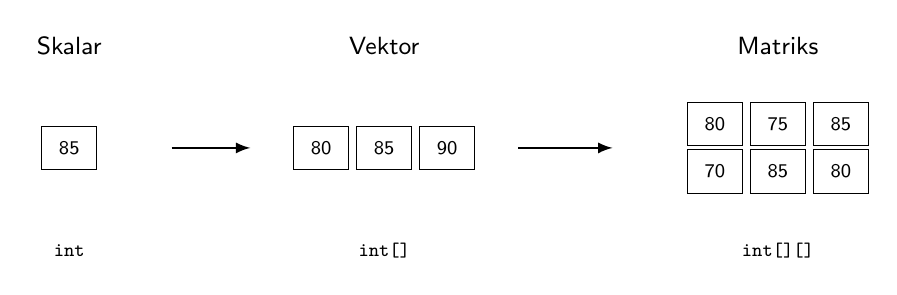
\begin{tikzpicture}[
			cell/.style={rectangle, draw=black, minimum width=0.7cm, minimum height=0.55cm, align=center, font=\scriptsize\sffamily}
		]
		\node[font=\sffamily\small] at (0, 1.3) {Skalar};
		\node[font=\ttfamily\scriptsize] at (0, -1.3) {int};
		\node[cell] at (0, 0) {85};

		\node[font=\sffamily\small] at (4, 1.3) {Vektor};
		\node[font=\ttfamily\scriptsize] at (4, -1.3) {int[]};
		\node[cell] at (3.2, 0) {80};
		\node[cell] at (4, 0) {85};
		\node[cell] at (4.8, 0) {90};

		\node[font=\sffamily\small] at (9, 1.3) {Matriks};
		\node[font=\ttfamily\scriptsize] at (9, -1.3) {int[][]};
		\node[cell] at (8.2, 0.3) {80};
		\node[cell] at (9, 0.3) {75};
		\node[cell] at (9.8, 0.3) {85};
		\node[cell] at (8.2, -0.3) {70};
		\node[cell] at (9, -0.3) {85};
		\node[cell] at (9.8, -0.3) {80};

		\draw[thick, -latex] (1.3, 0) -- (2.3, 0);
		\draw[thick, -latex] (5.7, 0) -- (6.9, 0);
	\end{tikzpicture}
	\caption{Hierarki skalar, vektor, dan matriks beserta padanan tipe data di pemrograman.}
	\label{fig:hierarki}
\end{figure}

Cara membaca Gambar~\ref{fig:hierarki}: gambar ini menampilkan tiga kelompok dari kiri ke kanan. Kelompok pertama berlabel Skalar dengan satu kotak berisi 85 dan tulisan \texttt{int} di bawah. Kelompok kedua berlabel Vektor dengan tiga kotak bersebelahan berisi 80, 85, 90 dan tulisan \texttt{int[]} di bawah. Kelompok ketiga berlabel Matriks dengan kotak-kotak tersusun dua baris tiga kolom berisi nilai 80, 75, 85 di atas dan 70, 85, 80 di bawah, dengan tulisan \texttt{int[][]} di bawahnya. Panah mengarah dari satu kelompok ke kelompok berikutnya untuk menunjukkan peningkatan dimensi. Inti pesan gambar ini adalah setiap penambahan dimensi membutuhkan satu tingkat tipe data tambahan di pemrograman.

\subsection{Cara Berpikir: Kapan Data Disebut Matriks}

Saat menghadapi data, ajukan tiga pertanyaan. Pertama, apakah data punya dua sumbu, misalnya baris dan kolom? Jika hanya satu sumbu, data itu vektor. Jika dua sumbu, data itu matriks. Kedua, apakah posisi dalam sumbu bermakna? Jika baris berarti mahasiswa dan kolom berarti mata kuliah, maka posisi bermakna. Ketiga, apakah semua baris punya jumlah kolom sama? Jika tidak, data itu bukan matriks persegi panjang yang bisa dioperasikan secara aljabar.

Jika ketiga pertanyaan itu dijawab, representasi data sudah pasti. Data akademik adalah matriks. Data urutan antrean adalah vektor. Data suhu setiap jam selama seminggu adalah matriks dengan baris hari dan kolom jam.

\subsection{Ringkasan}

Tabel~\ref{tab:matriks-programming} menyandingkan konsep matriks dengan pemrograman.

\begin{table}[H]
	\centering
	\caption{Padanan matriks dengan pemrograman.}
	\label{tab:matriks-programming}
	\small
	\begin{tabularx}{\textwidth}{l X X}
		\toprule
		Konsep  & Matematika               & Pemrograman                                     \\
		\midrule
		Skalar  & bilangan tunggal         & variabel \texttt{int}                           \\
		Vektor  & baris atau kolom tunggal & array satu dimensi                              \\
		Matriks & susunan baris dan kolom  & array dua dimensi                               \\
		Elemen  & $a_{ij}$                 & \texttt{M[i][j]}                                \\
		Ordo    & $m \times n$             & \texttt{M.length} $\times$ \texttt{M[0].length} \\
		\bottomrule
	\end{tabularx}
\end{table}

\section{Jenis-Jenis Matriks}

\subsection{Analogi: Bentuk Lemari yang Berbeda}

Lemari arsip punya berbagai bentuk. Ada lemari persegi dengan jumlah laci baris sama dengan jumlah laci kolom. Ada lemari sempit hanya satu kolom. Ada lemari panjang hanya satu baris. Ada lemari kosong tanpa dokumen. Ada lemari dengan satu dokumen besar di setiap laci diagonal. Ada lemari yang diputar sembilan puluh derajat sehingga baris menjadi kolom.

Enam bentuk itulah yang disebut jenis-jenis matriks.

\subsection{Enam Jenis Matriks}

Matriks persegi memiliki jumlah baris sama dengan jumlah kolom, misalnya $2 \times 2$. Vektor kolom hanya memiliki satu kolom, misalnya $3 \times 1$. Vektor baris hanya memiliki satu baris, misalnya $1 \times 3$. Matriks nol memiliki semua elemen bernilai 0. Matriks identitas $I_n$ adalah matriks persegi dengan elemen diagonal bernilai 1 dan elemen lain bernilai 0. Transpos $A^T$ adalah matriks yang diperoleh dengan menukar baris dan kolom, sehingga elemen $a_{ij}$ di $A$ menjadi $a_{ji}$ di $A^T$.

Keenam jenis itu ditunjukkan pada Gambar~\ref{fig:jenis-matriks}.

\begin{figure}[H]
	\centering
	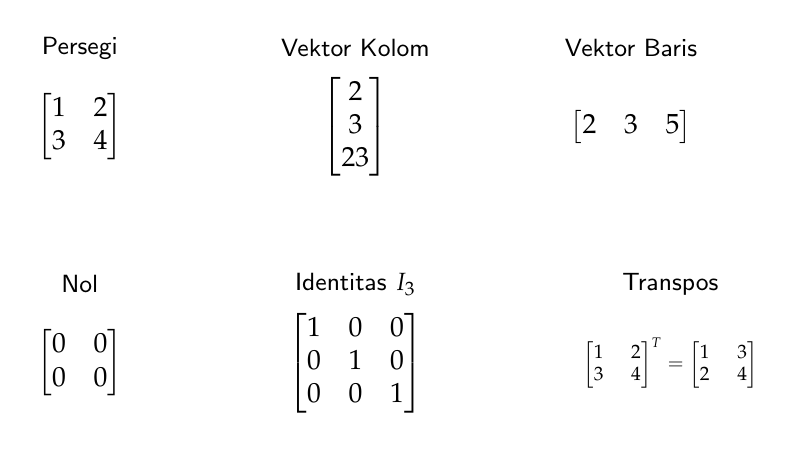
\begin{tikzpicture}[
			grp/.style={font=\sffamily\small, align=center},
			mat/.style={align=center, font=\sffamily}
		]
		\node[grp] at (0, 3.2) {Persegi};
		\node[mat] at (0, 2.2) {$\begin{bmatrix}1&2\\3&4\end{bmatrix}$};

		\node[grp] at (3.5, 3.2) {Vektor Kolom};
		\node[mat] at (3.5, 2.2) {$\begin{bmatrix}2\\3\\23\end{bmatrix}$};

		\node[grp] at (7, 3.2) {Vektor Baris};
		\node[mat] at (7, 2.2) {$\begin{bmatrix}2&3&5\end{bmatrix}$};

		\node[grp] at (0, 0.2) {Nol};
		\node[mat] at (0, -0.8) {$\begin{bmatrix}0&0\\0&0\end{bmatrix}$};

		\node[grp] at (3.5, 0.2) {Identitas $I_3$};
		\node[mat] at (3.5, -0.8) {$\begin{bmatrix}1&0&0\\0&1&0\\0&0&1\end{bmatrix}$};

		\node[grp] at (7.5, 0.2) {Transpos};
		\node[font=\scriptsize, align=center] at (7.5, -0.8) {$\begin{bmatrix}1&2\\3&4\end{bmatrix}^{T}=\begin{bmatrix}1&3\\2&4\end{bmatrix}$};
	\end{tikzpicture}
	\caption{Enam jenis matriks beserta contohnya.}
	\label{fig:jenis-matriks}
\end{figure}

Cara membaca Gambar~\ref{fig:jenis-matriks}: gambar ini menampilkan enam contoh matriks dalam susunan dua baris tiga kolom. Baris atas dari kiri ke kanan menampilkan matriks persegi $2 \times 2$, vektor kolom $3 \times 1$, dan vektor baris $1 \times 3$. Baris bawah dari kiri ke kanan menampilkan matriks nol $2 \times 2$, matriks identitas $I_3$, dan contoh transpos yang menunjukkan matriks $2 \times 2$ diubah menjadi transposnya dengan menukar baris dan kolom. Setiap contoh diberi label di atasnya. Inti pesan gambar ini adalah matriks punya bentuk-bentuk khusus yang punya nama, dan setiap bentuk punya kegunaan sendiri.

\subsection{Mengapa Ini Penting}

Matriks identitas berperan sebagai angka satu pada perkalian matriks. Jika $AI=IA=A$, maka $I$ adalah identitas perkalian. Konsep ini penting saat menghitung invers, karena $A^{-1}A=I$ adalah definisi resmi invers.

Matriks transpos dipakai di banyak algoritma. Saat menyimpan data tabel di basis data, transpos memungkinkan pengambilan data berdasarkan kolom tanpa harus menulis ulang query.

\subsection{Ringkasan}

Tabel~\ref{tab:jenis-matriks} merangkum keenam jenis matriks.

\begin{table}[H]
	\centering
	\caption{Ringkasan jenis-jenis matriks.}
	\label{tab:jenis-matriks}
	\small
	\begin{tabularx}{\textwidth}{l X X}
		\toprule
		Jenis        & Ciri                      & Contoh                                         \\
		\midrule
		Persegi      & baris $=$ kolom           & $\begin{smallmatrix}1&2\\3&4\end{smallmatrix}$ \\
		Vektor kolom & satu kolom                & $\begin{smallmatrix}2\\3\\23\end{smallmatrix}$ \\
		Vektor baris & satu baris                & $\begin{smallmatrix}2&3&5\end{smallmatrix}$    \\
		Nol          & semua elemen 0            & $\begin{smallmatrix}0&0\\0&0\end{smallmatrix}$ \\
		Identitas    & diagonal 1, lain 0        & $I_n$                                          \\
		Transpos     & $a_{ij}$ menjadi $a_{ji}$ & $A^T$                                          \\
		\bottomrule
	\end{tabularx}
\end{table}

\section{Kesamaan Matriks}

\subsection{Analogi: Dua Lemari yang Identik}

Dua lemari disebut identik jika punya jumlah laci yang sama di setiap baris dan setiap kolom, dan setiap laci bernomor sama berisi dokumen yang sama. Jika satu laci saja berbeda, kedua lemari tidak identik.

Kesamaan matriks juga begitu. Dua matriks disebut sama jika ordonya sama dan setiap elemen yang seletak bernilai sama. Jika ordonya berbeda, kedua matriks sudah pasti tidak sama, walaupun isi beberapa elemennya mirip.

\subsection{Contoh Berangka}

Diketahui $A=\begin{bmatrix}x&4\\7&y\end{bmatrix}$ dan $B=\begin{bmatrix}3&4\\7&9\end{bmatrix}$. Karena ordo $A$ sama dengan ordo $B$, kita tinggal mencocokkan elemen seletak. Elemen $a_{11}=x$ harus sama dengan $b_{11}=3$, sehingga $x=3$. Elemen $a_{22}=y$ harus sama dengan $b_{22}=9$, sehingga $y=9$. Elemen $a_{12}=4$, $a_{21}=7$, $b_{12}=4$, dan $b_{21}=7$ sudah cocok \cite{anton}.

\subsection{Cara Berpikir: Kesamaan sebagai Sistem Persamaan}

Kesamaan matriks sebenarnya adalah sistem persamaan linear yang ditulis dalam bentuk singkat. Setiap pasangan elemen seletak memberi satu persamaan. Jika ada empat pasang elemen, ada empat persamaan. Jika variabel yang dicari hanya dua, dua persamaan lain mungkin hanya berfungsi sebagai pemeriksa konsistensi.

\section{Operasi Dasar pada Matriks}

\subsection{Analogi: Menjumlahkan Dua Daftar Belanja}

Bayangkan dua daftar belanja yang isinya sama jenisnya: baris untuk barang, kolom untuk toko. Daftar pertama mencatat harga di toko A. Daftar kedua mencatat harga di toko B. Jika ingin tahu total harga jika membeli satu barang dari masing-masing toko, cukup jumlahkan setiap sel yang beralamat sama.

Penjumlahan matriks bekerja seperti itu. Dua matriks dijumlahkan dengan menjumlahkan elemen yang seletak, asalkan ordonya sama.

\subsection{Penjumlahan dan Pengurangan}

Jika $A=[a_{ij}]$ dan $B=[b_{ij}]$ memiliki ordo sama, maka $C=A+B$ didefinisikan sebagai $c_{ij}=a_{ij}+b_{ij}$. Pengurangan bekerja serupa: $c_{ij}=a_{ij}-b_{ij}$. Syaratnya satu: ordo $A$ harus sama dengan ordo $B$. Jika ordo berbeda, operasi tidak terdefinisi.

Contoh penjumlahan: $\begin{bmatrix}3&8\\4&6\end{bmatrix}+\begin{bmatrix}4&0\\1&-9\end{bmatrix}=\begin{bmatrix}7&8\\5&-3\end{bmatrix}$. Elemen $c_{11}=3+4=7$, $c_{12}=8+0=8$, $c_{21}=4+1=5$, $c_{22}=6+(-9)=-3$. Contoh pengurangan: $\begin{bmatrix}3&8\\4&6\end{bmatrix}-\begin{bmatrix}4&0\\1&-9\end{bmatrix}=\begin{bmatrix}-1&8\\3&15\end{bmatrix}$ \cite{lipschutz}. Perhatikan Gambar~\ref{fig:penjumlahan}.

\begin{figure}[H]
	\centering
	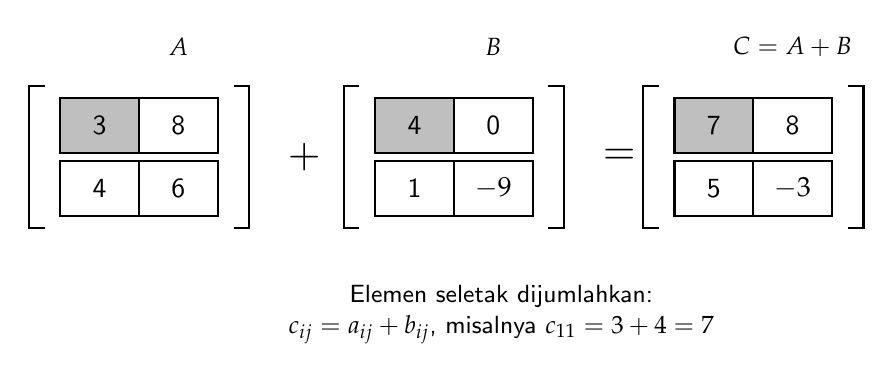
\begin{tikzpicture}[
			cell/.style={rectangle, draw=black, thick, minimum width=1.0cm, minimum height=0.7cm, align=center, font=\sffamily},
			hl/.style={cell, fill=black!25}
		]
		\node[font=\sffamily\small] at (-2.6, 1.6) {$A$};
		\node[hl] at (-3.6, 0.6) {3};
		\node[cell] at (-2.6, 0.6) {8};
		\node[cell] at (-3.6, -0.2) {4};
		\node[cell] at (-2.6, -0.2) {6};
		\draw[thick] (-4.3, 1.1) -- (-4.5, 1.1) -- (-4.5, -0.7) -- (-4.3, -0.7);
		\draw[thick] (-1.9, 1.1) -- (-1.7, 1.1) -- (-1.7, -0.7) -- (-1.9, -0.7);

		\node[font=\Large\sffamily] at (-1.0, 0.2) {$+$};

		\node[font=\sffamily\small] at (1.4, 1.6) {$B$};
		\node[hl] at (0.4, 0.6) {4};
		\node[cell] at (1.4, 0.6) {0};
		\node[cell] at (0.4, -0.2) {1};
		\node[cell] at (1.4, -0.2) {$-9$};
		\draw[thick] (-0.3, 1.1) -- (-0.5, 1.1) -- (-0.5, -0.7) -- (-0.3, -0.7);
		\draw[thick] (2.1, 1.1) -- (2.3, 1.1) -- (2.3, -0.7) -- (2.1, -0.7);

		\node[font=\Large\sffamily] at (3.0, 0.2) {$=$};

		\node[font=\sffamily\small] at (5.2, 1.6) {$C=A+B$};
		\node[hl] at (4.2, 0.6) {7};
		\node[cell] at (5.2, 0.6) {8};
		\node[cell] at (4.2, -0.2) {5};
		\node[cell] at (5.2, -0.2) {$-3$};
		\draw[thick] (3.5, 1.1) -- (3.3, 1.1) -- (3.3, -0.7) -- (3.5, -0.7);
		\draw[thick] (5.9, 1.1) -- (6.1, 1.1) -- (6.1, -0.7) -- (5.9, -0.7);

		\node[font=\small\sffamily, align=center] at (1.5, -1.8) {Elemen seletak dijumlahkan:\\$c_{ij}=a_{ij}+b_{ij}$, misalnya $c_{11}=3+4=7$};
	\end{tikzpicture}
	\caption{Penjumlahan dua matriks dengan elemen seletak dijumlahkan.}
	\label{fig:penjumlahan}
\end{figure}

Cara membaca Gambar~\ref{fig:penjumlahan}: gambar ini menampilkan tiga matriks berdampingan dari kiri ke kanan: matriks $A$, tanda tambah, matriks $B$, tanda sama dengan, dan matriks $C$. Setiap matriks punya empat sel yang tersusun dua baris dan dua kolom. Sel-sel yang saling berkorespondensi diberi latar abu-abu: sel kiri atas $A$ berisi 3, sel kiri atas $B$ berisi 4, dan sel kiri atas $C$ berisi 7. Di bawah gambar ada keterangan bahwa elemen seletak dijumlahkan dan $c_{11}=3+4=7$. Inti pesan gambar ini adalah penjumlahan matriks berjalan sel per sel pada alamat yang sama.

\subsection{Perkalian Skalar}

Perkalian skalar adalah perkalian setiap elemen matriks dengan satu bilangan real $k$. Jika $A=[a_{ij}]$, maka $kA=[ka_{ij}]$. Contoh: $3 \cdot \begin{bmatrix}1&2\\3&4\end{bmatrix}=\begin{bmatrix}3&6\\9&12\end{bmatrix}$. Semua elemen dikalikan dengan 3 \cite{anton}.

\subsection{Kalau Salah: Perkalian Skalar yang Ditafsirkan Sebagai Pangkat}

Kesalahan umum terjadi ketika melihat $2 \cdot A$ dan mengira hasilnya adalah matriks $A$ yang dikalikan dengan dirinya sendiri. Itu salah. Perkalian skalar mengalikan setiap elemen dengan skalar. Perpangkatan matriks $A^2=AA$ melakukan perkalian matriks dengan dirinya sendiri, yang hasilnya berbeda. Pada matriks $A=\begin{bmatrix}1&2\\3&4\end{bmatrix}$, perkalian skalar $2A=\begin{bmatrix}2&4\\6&8\end{bmatrix}$, sedangkan perpangkatan $A^2=\begin{bmatrix}7&10\\15&22\end{bmatrix}$. Keduanya tidak sama.

\subsection{Ringkasan}

Tabel~\ref{tab:operasi-dasar} merangkum tiga operasi dasar.

\begin{table}[H]
	\centering
	\caption{Ringkasan operasi dasar matriks.}
	\label{tab:operasi-dasar}
	\small
	\begin{tabularx}{\textwidth}{l X X}
		\toprule
		Operasi          & Syarat              & Aturan                  \\
		\midrule
		Penjumlahan      & ordo $A$ = ordo $B$ & $c_{ij}=a_{ij}+b_{ij}$  \\
		Pengurangan      & ordo $A$ = ordo $B$ & $c_{ij}=a_{ij}-b_{ij}$  \\
		Perkalian skalar & selalu bisa         & $c_{ij}=k \cdot a_{ij}$ \\
		\bottomrule
	\end{tabularx}
\end{table}

\section{Perkalian Matriks}

\subsection{Analogi: Merangkai Baris dan Kolom}

Bayangkan dua papan tombol. Papan pertama punya tiga tombol per baris. Papan kedua punya tiga tombol per kolom. Untuk memindahkan sinyal dari papan pertama ke papan kedua, setiap baris di papan pertama harus bertemu dengan satu kolom di papan kedua, lalu dikalikan elemen per elemen dan dijumlahkan. Hasilnya satu angka.

Itulah perkalian matriks. Setiap elemen hasil adalah jumlah hasil kali elemen satu baris di matriks pertama dengan elemen satu kolom di matriks kedua.

\subsection{Syarat Perkalian}

Perkalian $AB$ hanya terdefinisi jika jumlah kolom $A$ sama dengan jumlah baris $B$. Jika $A$ berordo $m \times n$ dan $B$ berordo $n \times p$, maka hasil $C=AB$ berordo $m \times p$. Perhatikan Gambar~\ref{fig:syarat-perkalian}.

\begin{figure}[H]
	\centering
	\begin{tikzpicture}[
			dim/.style={font=\small\sffamily, align=center},
			big/.style={font=\Large\sffamily}
		]
		\node[font=\sffamily\small] at (0, 2.5) {Valid:};
		\node[dim] at (0, 1.5) {$A_{2\times 3}$};
		\node[big] at (1.8, 1.5) {$\times$};
		\node[dim] at (3.6, 1.5) {$B_{3\times 2}$};
		\node[big] at (5.4, 1.5) {$=$};
		\node[dim] at (7.2, 1.5) {$C_{2\times 2}$};

		\draw[thick] (0.4, 0.9) -- (0.4, 0.6) -- (1.3, 0.6) -- (1.3, 0.9);
		\draw[thick] (3.2, 0.9) -- (3.2, 0.6) -- (2.3, 0.6) -- (2.3, 0.9);
		\node[font=\scriptsize\sffamily] at (1.8, 0.35) {sama: 3};

		\draw[thick, -latex] (-0.4, 0.9) -- (-0.4, -0.4) -- (7.2, -0.4) -- (7.2, 0.9);
		\node[font=\scriptsize\sffamily, fill=white] at (3.4, -0.4) {hasil: 2 baris $\times$ 2 kolom};

		\node[font=\sffamily\small] at (0, -2.0) {Tidak valid:};
		\node[dim] at (0, -3.0) {$A_{2\times 3}$};
		\node[big] at (1.8, -3.0) {$\times$};
		\node[dim] at (3.6, -3.0) {$B_{2\times 3}$};
		\node[big] at (5.4, -3.0) {$\neq$};
		\node[dim] at (7.2, -3.0) {tidak terdefinisi};

		\node[font=\scriptsize\sffamily, align=center] at (1.8, -3.9) {3 $\neq$ 2\\(kolom $A$ $\neq$ baris $B$)};
	\end{tikzpicture}
	\caption{Syarat perkalian matriks: jumlah kolom $A$ harus sama dengan jumlah baris $B$.}
	\label{fig:syarat-perkalian}
\end{figure}

Cara membaca Gambar~\ref{fig:syarat-perkalian}: gambar ini menampilkan dua contoh berdampingan. Contoh atas berlabel "Valid" dengan tiga simbol $A_{2\times 3}$, $\times$, $B_{3\times 2}$, $=$, $C_{2\times 2}$. Di bawah $A$ dan $B$ ada garis penghubung yang menunjukkan bahwa angka 3 (kolom $A$) sama dengan angka 3 (baris $B$). Garis lain mengarah dari sisi luar ke hasil, menunjukkan bahwa 2 baris $A$ dan 2 kolom $B$ menjadi ordo hasil. Contoh bawah berlabel "Tidak valid" dengan $A_{2\times 3}$ dan $B_{2\times 3}$ yang tidak menghasilkan matriks, karena angka 3 tidak sama dengan 2. Inti pesan gambar ini adalah syarat perkalian hanya bergantung pada kesesuaian dua dimensi dalam.

\subsection{Cara Menghitung Elemen Hasil}

Setiap elemen $c_{ij}$ adalah jumlah hasil kali elemen baris $i$ matriks $A$ dengan elemen kolom $j$ matriks $B$. Jika $A=\begin{bmatrix}1&2&3\\4&5&6\end{bmatrix}$ dan $B=\begin{bmatrix}7&8\\9&10\\11&12\end{bmatrix}$, maka $C=AB$ dihitung sebagai berikut.

Elemen $c_{11}$ adalah $(1)(7)+(2)(9)+(3)(11)=7+18+33=58$.

Elemen $c_{12}$ adalah $(1)(8)+(2)(10)+(3)(12)=8+20+36=64$.

Elemen $c_{21}$ adalah $(4)(7)+(5)(9)+(6)(11)=28+45+66=139$.

Elemen $c_{22}$ adalah $(4)(8)+(5)(10)+(6)(12)=32+50+72=154$.

Jadi $C=\begin{bmatrix}58&64\\139&154\end{bmatrix}$ \cite{lipschutz}. Perhatikan Gambar~\ref{fig:dot-product}.

\begin{figure}[H]
	\centering
	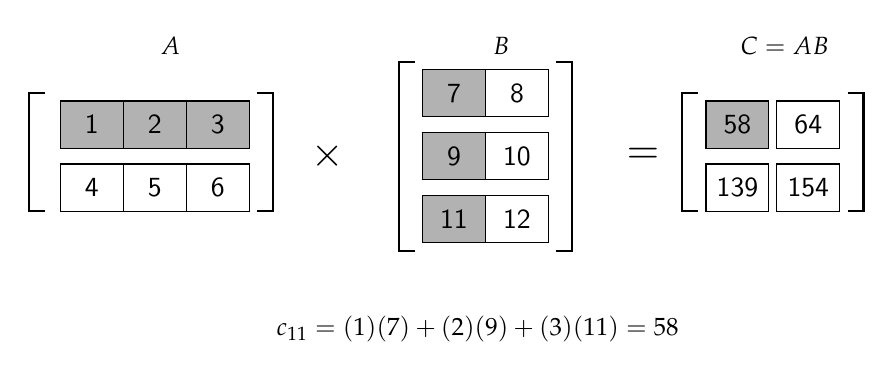
\begin{tikzpicture}[
			cell/.style={rectangle, draw=black, minimum width=0.8cm, minimum height=0.6cm, align=center, font=\sffamily},
			hl/.style={cell, fill=black!30}
		]
		\node[font=\sffamily\small] at (-2.4, 1.5) {$A$};
		\node[hl] at (-3.4, 0.5) {1};
		\node[hl] at (-2.6, 0.5) {2};
		\node[hl] at (-1.8, 0.5) {3};
		\node[cell] at (-3.4, -0.3) {4};
		\node[cell] at (-2.6, -0.3) {5};
		\node[cell] at (-1.8, -0.3) {6};
		\draw[thick] (-4.0, 0.9) -- (-4.2, 0.9) -- (-4.2, -0.6) -- (-4.0, -0.6);
		\draw[thick] (-1.3, 0.9) -- (-1.1, 0.9) -- (-1.1, -0.6) -- (-1.3, -0.6);

		\node[font=\Large\sffamily] at (-0.4, 0.1) {$\times$};

		\node[font=\sffamily\small] at (1.8, 1.5) {$B$};
		\node[hl] at (1.2, 0.9) {7};
		\node[cell] at (2.0, 0.9) {8};
		\node[hl] at (1.2, 0.1) {9};
		\node[cell] at (2.0, 0.1) {10};
		\node[hl] at (1.2, -0.7) {11};
		\node[cell] at (2.0, -0.7) {12};
		\draw[thick] (0.7, 1.3) -- (0.5, 1.3) -- (0.5, -1.1) -- (0.7, -1.1);
		\draw[thick] (2.5, 1.3) -- (2.7, 1.3) -- (2.7, -1.1) -- (2.5, -1.1);

		\node[font=\Large\sffamily] at (3.6, 0.1) {$=$};

		\node[font=\sffamily\small] at (5.4, 1.5) {$C=AB$};
		\node[hl] at (4.8, 0.5) {58};
		\node[cell] at (5.7, 0.5) {64};
		\node[cell] at (4.8, -0.3) {139};
		\node[cell] at (5.7, -0.3) {154};
		\draw[thick] (4.3, 0.9) -- (4.1, 0.9) -- (4.1, -0.6) -- (4.3, -0.6);
		\draw[thick] (6.2, 0.9) -- (6.4, 0.9) -- (6.4, -0.6) -- (6.2, -0.6);

		\node[font=\small\sffamily, align=center] at (1.5, -2.1) {$c_{11}=(1)(7)+(2)(9)+(3)(11)=58$};
	\end{tikzpicture}
	\caption{Perkalian matriks dengan baris $A$ bertemu kolom $B$.}
	\label{fig:dot-product}
\end{figure}

Cara membaca Gambar~\ref{fig:dot-product}: gambar ini menampilkan tiga matriks dari kiri ke kanan: matriks $A$, tanda kali, matriks $B$, tanda sama dengan, dan matriks $C$. Pada matriks $A$, baris pertama (1, 2, 3) diberi latar abu-abu gelap. Pada matriks $B$, kolom pertama (7, 9, 11) juga diberi latar abu-abu gelap. Pada matriks $C$, sel kiri atas yang berisi 58 diberi latar abu-abu gelap yang sama. Di bawah gambar ada rumus $c_{11}=(1)(7)+(2)(9)+(3)(11)=58$. Inti pesan gambar ini adalah elemen hasil $c_{ij}$ berasal dari satu baris $A$ dan satu kolom $B$ yang dipasangkan elemen per elemen lalu dijumlahkan.

\subsection{Kalau Salah: Perkalian Elemen per Elemen}

Kesalahan paling sering adalah mengalikan matriks dengan mengalikan elemen seletak, seperti penjumlahan. Jika begitu, hasilnya bukan $C$ yang benar. Dengan $A$ dan $B$ yang sama seperti di atas, perkalian seletak akan menghasilkan $\begin{bmatrix}1 \cdot 7&2 \cdot 8\\4 \cdot 9&5 \cdot 10\\6 \cdot 11&?\end{bmatrix}$ yang bahkan tidak bisa dibentuk karena ordonya tidak cocok.

Perkalian matriks memakai aturan baris kali kolom, bukan elemen kali elemen. Perkalian elemen per elemen memang ada di matematika, tetapi namanya berbeda: perkalian Hadamard, dan hanya terdefinisi jika kedua matriks berordo sama.

\subsection{Ringkasan}

Tabel~\ref{tab:perkalian} merangkum aturan perkalian matriks.

\begin{table}[H]
	\centering
	\caption{Ringkasan perkalian matriks.}
	\label{tab:perkalian}
	\small
	\begin{tabularx}{\textwidth}{l X X}
		\toprule
		Aspek  & Aturan                               & Contoh                                      \\
		\midrule
		Syarat & kolom $A$ = baris $B$                & $A_{2\times 3} \cdot B_{3\times 2}$ sah     \\
		Hasil  & $m$ baris $A$ $\times$ $p$ kolom $B$ & $C_{2\times 2}$                             \\
		Elemen & $c_{ij}=\sum_{k} a_{ik} b_{kj}$      & $c_{11}=1 \cdot 7 + 2 \cdot 9 + 3 \cdot 11$ \\
		Bukan  & perkalian seletak                    & hanya berlaku bila ordo sama                \\
		\bottomrule
	\end{tabularx}
\end{table}

\section{Determinan}

\subsection{Analogi: Sidik Jari Matriks}

Setiap matriks persegi punya sidik jari berupa satu bilangan yang disebut determinan. Sidik jari ini menentukan apakah matriks itu bisa dibalik atau tidak. Jika determinan nol, matriks tidak punya invers. Jika determinan bukan nol, matriks punya invers.

Determinan ditulis $\det(A)$ atau $|A|$. Untuk matriks kecil, sidik jari ini dihitung dengan rumus sederhana. Untuk matriks besar, sidik jari dihitung dengan mengurangi pekerjaan menjadi submasalah yang lebih kecil.

\subsection{Determinan 2$\times$2}

Untuk matriks $A=\begin{bmatrix}a&b\\c&d\end{bmatrix}$, determinannya adalah $ad-bc$. Contoh: $B=\begin{bmatrix}4&6\\3&8\end{bmatrix}$ memiliki $\det(B)=(4)(8)-(6)(3)=32-18=14$ \cite{anton}. Perhatikan Gambar~\ref{fig:determinan-2x2}.

\begin{figure}[H]
	\centering
	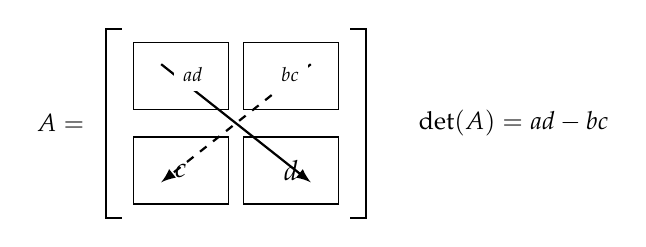
\begin{tikzpicture}[
			cell/.style={rectangle, draw=black, minimum width=1.2cm, minimum height=0.85cm, align=center, font=\sffamily}
		]
		\node[cell] (a) at (0, 0.7) {$a$};
		\node[cell] (b) at (1.4, 0.7) {$b$};
		\node[cell] (c) at (0, -0.5) {$c$};
		\node[cell] (d) at (1.4, -0.5) {$d$};

		\draw[thick] (-0.75, 1.3) -- (-0.95, 1.3) -- (-0.95, -1.1) -- (-0.75, -1.1);
		\draw[thick] (2.15, 1.3) -- (2.35, 1.3) -- (2.35, -1.1) -- (2.15, -1.1);

		\node[font=\sffamily\small, anchor=east] at (-1.1, 0.1) {$A=$};

		\draw[thick, -latex] (-0.25, 0.85) -- (1.65, -0.65);
		\node[font=\scriptsize\sffamily, anchor=south east, fill=white] at (0.4, 0.5) {$ad$};

		\draw[thick, dashed, -latex] (1.65, 0.85) -- (-0.25, -0.65);
		\node[font=\scriptsize\sffamily, anchor=south west, fill=white] at (1.15, 0.5) {$bc$};

		\node[font=\small\sffamily, anchor=west] at (2.9, 0.1) {$\det(A)=ad-bc$};
	\end{tikzpicture}
	\caption{Determinan matriks $2 \times 2$ dengan dua diagonal.}
	\label{fig:determinan-2x2}
\end{figure}

Cara membaca Gambar~\ref{fig:determinan-2x2}: gambar ini menampilkan matriks $2 \times 2$ dengan empat sel $a$, $b$, $c$, $d$. Ada dua panah: panah penuh dari $a$ ke $d$ mewakili diagonal utama $ad$, dan panah putus-putus dari $b$ ke $c$ mewakili diagonal kedua $bc$. Di sebelah kanan ada rumus $\det(A)=ad-bc$. Inti pesan gambar ini adalah determinan $2 \times 2$ adalah selisih dua hasil kali diagonal.

\subsection{Determinan 3$\times$3 dengan Aturan Sarrus}

Untuk matriks $A=\begin{bmatrix}a&b&c\\d&e&f\\g&h&i\end{bmatrix}$, determinannya dihitung dengan menyalin dua kolom pertama ke kanan, lalu menjumlahkan tiga hasil kali diagonal penuh dan mengurangkan tiga hasil kali diagonal putus.

Rumusnya: $\det(A)=a(ei-fh)-b(di-fg)+c(dh-eg)$, atau ekuivalen dengan $(aei+bfg+cdh)-(ceg+afh+bdi)$ \cite{anton}. Perhatikan Gambar~\ref{fig:sarrus}.

\begin{figure}[H]
	\centering
	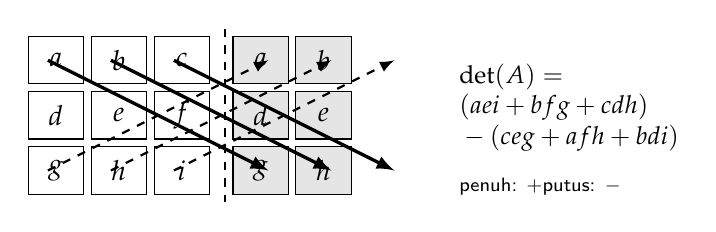
\begin{tikzpicture}[
			cell/.style={rectangle, draw=black, minimum width=0.7cm, minimum height=0.6cm, align=center, font=\sffamily},
			rep/.style={cell, fill=black!10}
		]
		\node[cell] at (0, 1.0) {$a$};
		\node[cell] at (0.8, 1.0) {$b$};
		\node[cell] at (1.6, 1.0) {$c$};
		\node[cell] at (0, 0.3) {$d$};
		\node[cell] at (0.8, 0.3) {$e$};
		\node[cell] at (1.6, 0.3) {$f$};
		\node[cell] at (0, -0.4) {$g$};
		\node[cell] at (0.8, -0.4) {$h$};
		\node[cell] at (1.6, -0.4) {$i$};

		\node[rep] at (2.6, 1.0) {$a$};
		\node[rep] at (3.4, 1.0) {$b$};
		\node[rep] at (2.6, 0.3) {$d$};
		\node[rep] at (3.4, 0.3) {$e$};
		\node[rep] at (2.6, -0.4) {$g$};
		\node[rep] at (3.4, -0.4) {$h$};

		\draw[thick, dashed] (2.15, 1.4) -- (2.15, -0.8);

		\draw[very thick, -latex] (-0.1, 1.0) -- (2.7, -0.4);
		\draw[very thick, -latex] (0.7, 1.0) -- (3.5, -0.4);
		\draw[very thick, -latex] (1.5, 1.0) -- (4.3, -0.4);

		\draw[thick, dashed, -latex] (-0.1, -0.4) -- (2.7, 1.0);
		\draw[thick, dashed, -latex] (0.7, -0.4) -- (3.5, 1.0);
		\draw[thick, dashed, -latex] (1.5, -0.4) -- (4.3, 1.0);

		\node[font=\small\sffamily, anchor=west, align=left] at (5.0, 0.4) {
			$\det(A)=$\\
			$\phantom{}(aei+bfg+cdh)$\\
			$\phantom{}-(ceg+afh+bdi)$
		};
		\node[font=\scriptsize\sffamily, anchor=west] at (5.0, -0.6) {penuh: $+$\\putus: $-$};
	\end{tikzpicture}
	\caption{Determinan matriks $3\times 3$ dengan aturan Sarrus.}
	\label{fig:sarrus}
\end{figure}

Cara membaca Gambar~\ref{fig:sarrus}: gambar ini menampilkan matriks $3 \times 3$ dengan dua kolom pertama disalin ulang di kanannya, dipisahkan oleh garis putus-putus vertikal. Kolom yang disalin diberi latar abu-abu muda. Ada enam panah diagonal. Tiga panah penuh mengarah ke bawah-kanan mewakili hasil kali $aei$, $bfg$, dan $cdh$. Tiga panah putus-putus mengarah ke atas-kanan mewakili hasil kali $ceg$, $afh$, dan $bdi$. Di sebelah kanan ada rumus dengan tiga suku positif dan tiga suku negatif. Inti pesan gambar ini adalah penyalinan dua kolom memungkinkan enam diagonal lengkap digambar tanpa keluar dari batas matriks.

\subsection{Determinan 4$\times$4 dengan Ekspansi Kofaktor}

Untuk matriks berukuran lebih dari $3 \times 3$, aturan Sarrus tidak berlaku. Metode yang dipakai adalah ekspansi kofaktor pada baris pertama. Setiap elemen baris pertama dikalikan determinan submatriks yang tersisa setelah menghapus baris dan kolomnya, dengan tanda berselang-seling $+$, $-$, $+$, $-$.

Untuk matriks $A_{4 \times 4}$, $\det(A)=a \cdot M_{11}-b \cdot M_{12}+c \cdot M_{13}-d \cdot M_{14}$, dengan $M_{1j}$ adalah determinan submatriks $3\times 3$ hasil penghapusan baris 1 dan kolom $j$ \cite{anton}.

\subsection{Mengapa Determinan Penting}

Determinan menentukan apakah matriks punya invers. Jika $\det(A)=0$, matriks disebut singular dan tidak punya invers. Jika $\det(A) \ne 0$, matriks disebut non-singular dan punya invers. Determinan juga muncul saat menyelesaikan sistem persamaan linear dengan aturan Cramer, dan saat menghitung perubahan volume saat matriks diperlakukan sebagai transformasi geometri.

\section{Invers Matriks}

\subsection{Analogi: Pembagian pada Matriks}

Pada bilangan biasa, jika $8x=40$, kita mencari $x$ dengan membagi 40 dengan 8. Pembagian itu ekuivalen dengan mengalikan 40 dengan kebalikan 8, yaitu $1/8$. Hasilnya $x=40 \times (1/8)=5$.

Pada matriks, jika $AX=B$, kita mencari $X$ dengan mengalikan kedua sisi dengan $A^{-1}$, yaitu kebalikan dari $A$. Hasilnya $X=A^{-1}B$. Invers adalah analog dari kebalikan. Perhatikan Gambar~\ref{fig:analogi-invers}.

\begin{figure}[H]
	\centering
	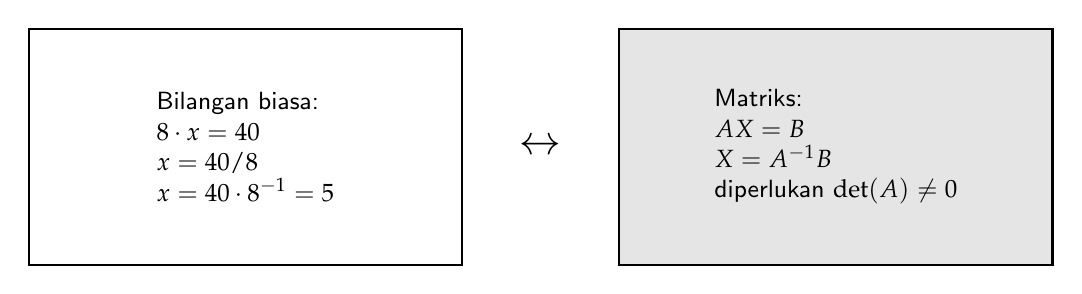
\begin{tikzpicture}[
			box/.style={rectangle, draw=black, thick, minimum width=5.5cm, minimum height=3cm, align=left, font=\sffamily\small, inner sep=10pt}
		]
		\node[box, fill=white] at (0, 0) {
			Bilangan biasa:\\
			$8 \cdot x=40$\\
			$x=40/8$\\
			$x=40 \cdot 8^{-1}=5$
		};
		\node[box, fill=black!10] at (7.5, 0) {
			Matriks:\\
			$AX=B$\\
			$X=A^{-1}B$\\
			diperlukan $\det(A) \neq 0$
		};

		\node[font=\Large\sffamily] at (3.75, 0) {$\leftrightarrow$};
	\end{tikzpicture}
	\caption{Analogi antara pembagian bilangan dan invers matriks.}
	\label{fig:analogi-invers}
\end{figure}

Cara membaca Gambar~\ref{fig:analogi-invers}: gambar ini menampilkan dua kotak sejajar. Kotak kiri berisi persamaan bilangan biasa $8x=40$ dengan solusi $x=40/8=40 \cdot 8^{-1}=5$. Kotak kanan berisi persamaan matriks $AX=B$ dengan solusi $X=A^{-1}B$. Di antara dua kotak ada panah bolak-balik. Kotak kiri berlatar putih dan kotak kanan berlatar abu-abu muda. Inti pesan gambar ini adalah invers matriks adalah analog dari kebalikan bilangan, dan keduanya memerlukan nilai yang bukan nol.

\subsection{Syarat Invers}

Matriks persegi $A$ punya invers $A^{-1}$ jika dan hanya jika $\det(A) \ne 0$. Jika ada, invers itu tunggal dan memenuhi $A^{-1}A=I$ dan $AA^{-1}=I$.

\subsection{Invers Matriks 2$\times$2}

Untuk matriks $A=\begin{bmatrix}a&b\\c&d\end{bmatrix}$, inversnya adalah $A^{-1}=\frac{1}{ad-bc}\begin{bmatrix}d&-b\\-c&a\end{bmatrix}$. Perhatikan urutan: diagonal utama $a,d$ bertukar posisi, diagonal kedua $b,c$ berubah tanda, dan seluruh matriks dibagi dengan determinan \cite{anton}.

Contoh: $A=\begin{bmatrix}4&7\\2&6\end{bmatrix}$ memiliki $\det(A)=(4)(6)-(7)(2)=24-14=10$. Maka $A^{-1}=\frac{1}{10}\begin{bmatrix}6&-7\\-2&4\end{bmatrix}=\begin{bmatrix}0{,}6&-0{,}7\\-0{,}2&0{,}4\end{bmatrix}$. Periksa dengan $A \cdot A^{-1}=\begin{bmatrix}1&0\\0&1\end{bmatrix}$ \cite{lipschutz}.

\subsection{Invers Matriks 3$\times$3}

Untuk matriks $3 \times 3$ atau lebih besar, invers dihitung dengan lima langkah berurutan. Langkah pertama hitung determinan. Jika nol, berhenti. Langkah kedua hitung minor $M_{ij}$ setiap elemen, yaitu determinan submatriks setelah menghapus baris $i$ dan kolom $j$. Langkah ketiga hitung kofaktor $C_{ij}=(-1)^{i+j} M_{ij}$, dengan tanda berselang-seling. Langkah keempat bentuk adjugate, yaitu transpos matriks kofaktor. Langkah kelima bagi adjugate dengan determinan: $A^{-1}=\frac{1}{\det(A)}\text{adj}(A)$ \cite{anton}. Alur langkah ini ditunjukkan pada Gambar~\ref{fig:alur-invers}.

\begin{figure}[H]
	\centering
	\begin{tikzpicture}[
			step/.style={rectangle, draw=black, thick, fill=black!5, minimum width=2.8cm, minimum height=0.9cm, align=center, font=\sffamily\small},
			arr/.style={draw, thick, -latex}
		]
		\node[step] (s1) at (0, 1.5) {1. Determinan};
		\node[step] (s2) at (3.4, 1.5) {2. Minor};
		\node[step] (s3) at (6.8, 1.5) {3. Kofaktor};
		\node[step] (s4) at (6.8, 0) {4. Adjugate};
		\node[step] (s5) at (3.4, 0) {5. Invers};

		\draw[arr] (s1) -- (s2);
		\draw[arr] (s2) -- (s3);
		\draw[arr] (s3) -- (s4);
		\draw[arr] (s4) -- (s5);
	\end{tikzpicture}
	\caption{Alur lima langkah menghitung invers matriks $3 \times 3$.}
	\label{fig:alur-invers}
\end{figure}

Cara membaca Gambar~\ref{fig:alur-invers}: gambar ini menampilkan lima kotak yang tersusun dalam pola dua baris. Baris atas dari kiri ke kanan berisi "Determinan", "Minor", dan "Kofaktor". Baris bawah dari kanan ke kiri berisi "Adjugate" di bawah Kofaktor, lalu "Invers" di bawah Minor. Panah mengarah dari Determinan ke Minor, dari Minor ke Kofaktor, dari Kofaktor turun ke Adjugate, dan dari Adjugate ke Invers. Inti pesan gambar ini adalah invers dihitung melalui lima langkah berurutan, dan setiap langkah bergantung pada hasil langkah sebelumnya.

\subsection{Contoh Invers 3$\times$3}

Diketahui $A=\begin{bmatrix}2&3&1\\1&2&1\\3&1&2\end{bmatrix}$. Hitung determinannya: $\det(A)=2(4-1)-3(2-3)+1(1-6)=2(3)-3(-1)+1(-5)=6+3-5=4$. Karena $4 \ne 0$, invers ada.

Minor setiap elemen dihitung dengan menghapus baris dan kolomnya. Minor $M_{11}$ adalah determinan submatriks $\begin{bmatrix}2&1\\1&2\end{bmatrix}$, yaitu $4-1=3$. Minor $M_{12}$ adalah determinan submatriks $\begin{bmatrix}1&1\\3&2\end{bmatrix}$, yaitu $2-3=-1$. Lanjutkan langkah serupa untuk semua sembilan elemen, menghasilkan matriks minor $M=\begin{bmatrix}3&-1&-5\\5&1&-1\\1&1&1\end{bmatrix}$.

Kofaktor diperoleh dengan menerapkan tanda berselang-seling. Tanda untuk $3 \times 3$ adalah $\begin{bmatrix}+&-&+\\-&+&-\\+&-&+\end{bmatrix}$. Setelah dikalikan tanda, matriks kofaktor menjadi $C=\begin{bmatrix}3&1&-5\\-5&1&1\\1&-1&1\end{bmatrix}$.

Adjugate adalah transpos kofaktor: $\text{adj}(A)=C^T=\begin{bmatrix}3&-5&1\\1&1&-1\\-5&1&1\end{bmatrix}$.

Invers adalah adjugate dibagi determinan: $A^{-1}=\frac{1}{4}\begin{bmatrix}3&-5&1\\1&1&-1\\-5&1&1\end{bmatrix}=\begin{bmatrix}0{,}75&-1{,}25&0{,}25\\0{,}25&0{,}25&-0{,}25\\-1{,}25&0{,}25&0{,}25\end{bmatrix}$.

\subsection{Kalau Salah: Invers Tanpa Cek Determinan}

Kesalahan paling sering adalah mencoba menghitung invers tanpa lebih dahulu memeriksa determinan. Jika determinan nol, rumus invers akan meminta pembagian dengan nol, yang tidak terdefinisi. Hasilnya bukan matriks salah, melainkan kegagalan komputasi yang bisa membuat program berhenti.

Contoh matriks dengan determinan nol adalah $\begin{bmatrix}1&2\\2&4\end{bmatrix}$. Determinan $=1(4)-2(2)=0$. Matriks ini tidak punya invers. Jika program tetap mencoba membaginya, akan muncul kesalahan pembagian dengan nol.

\subsection{Ringkasan}

Tabel~\ref{tab:invers} merangkum invers untuk berbagai ukuran.

\begin{table}[H]
	\centering
	\caption{Ringkasan invers matriks.}
	\label{tab:invers}
	\small
	\begin{tabularx}{\textwidth}{l X X}
		\toprule
		Ukuran       & Rumus                                                           & Langkah kunci                                   \\
		\midrule
		$2 \times 2$ & $\frac{1}{ad-bc}\begin{smallmatrix}d&-b\\-c&a\end{smallmatrix}$ & tukar diagonal utama, ubah tanda diagonal kedua \\
		$3 \times 3$ & $\frac{1}{\det(A)}\text{adj}(A)$                                & minor, kofaktor, transpos                       \\
		Syarat       & $\det(A) \ne 0$                                                 & periksa sebelum menghitung                      \\
		Identitas    & $A^{-1}A=I$                                                     & pemeriksa hasil                                 \\
		\bottomrule
	\end{tabularx}
\end{table}

\section{Studi Kasus}

\subsection{Studi Kasus 1: Nilai Akhir Mahasiswa}

\subsubsection{Langkah 1: Kumpulkan Data Mentah}

Sebuah sistem akademik mencatat nilai tiga mahasiswa pada tiga mata kuliah. Data mentahnya adalah tabel berikut. Andi mendapat 80, 75, 85. Budi mendapat 70, 85, 80. Citra mendapat 90, 80, 75. Urutan kolom adalah Matematika, Struktur Data, dan Pemrograman.

\subsubsection{Langkah 2: Bentuk Matriks Data}

Susun data menjadi matriks $M_{3 \times 3}$ dengan baris untuk mahasiswa dan kolom untuk mata kuliah. Matriksnya adalah $M=\begin{bmatrix}80&75&85\\70&85&80\\90&80&75\end{bmatrix}$. Baris pertama milik Andi, baris kedua milik Budi, baris ketiga milik Citra.

\subsubsection{Langkah 3: Definisikan Bobot sebagai Vektor Kolom}

Bobot mata kuliah adalah 40 persen Matematika, 30 persen Struktur Data, dan 30 persen Pemrograman. Susun bobot menjadi vektor kolom $W_{3 \times 1}=\begin{bmatrix}0{,}4\\0{,}3\\0{,}3\end{bmatrix}$. Vektor kolom dipilih karena setiap barisnya mewakili satu mata kuliah yang akan dipasangkan dengan satu kolom di matriks $M$.

\subsubsection{Langkah 4: Periksa Syarat Perkalian}

Matriks $M$ berordo $3 \times 3$, vektor $W$ berordo $3 \times 1$. Jumlah kolom $M$ adalah 3. Jumlah baris $W$ adalah 3. Syarat perkalian terpenuhi. Hasil $N=MW$ akan berordo $3 \times 1$, yaitu tiga nilai akhir untuk tiga mahasiswa.

\subsubsection{Langkah 5: Hitung Elemen Hasil Pertama}

Nilai akhir Andi adalah baris pertama $M$ dikali kolom $W$: $n_{11}=(80)(0{,}4)+(75)(0{,}3)+(85)(0{,}3)=32+22{,}5+25{,}5=80{,}0$.

\subsubsection{Langkah 6: Hitung Elemen Hasil Kedua dan Ketiga}

Nilai akhir Budi adalah baris kedua $M$ dikali $W$: $n_{21}=(70)(0{,}4)+(85)(0{,}3)+(80)(0{,}3)=28+25{,}5+24=77{,}5$. Nilai akhir Citra adalah baris ketiga $M$ dikali $W$: $n_{31}=(90)(0{,}4)+(80)(0{,}3)+(75)(0{,}3)=36+24+22{,}5=82{,}5$.

\subsubsection{Langkah 7: Susun Hasil}

Hasil lengkap adalah $N=\begin{bmatrix}80{,}0\\77{,}5\\82{,}5\end{bmatrix}$. Nilai tertinggi diperoleh Citra, disusul Andi, lalu Budi. Visualisasi alur data ditunjukkan pada Gambar~\ref{fig:nilai-akhir}.

\begin{figure}[H]
	\centering
	\resizebox{\textwidth}{!}{%
		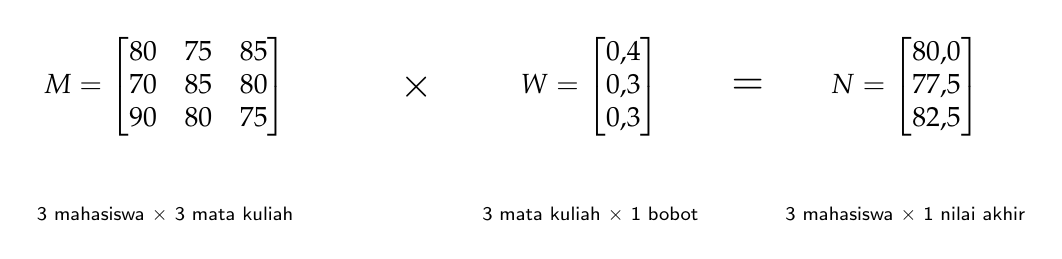
\begin{tikzpicture}[
				mat/.style={align=center, font=\sffamily}
			]
			\node[mat] (M) at (0,0) {$M=\begin{bmatrix}80&75&85\\70&85&80\\90&80&75\end{bmatrix}$};
			\node[font=\Large\sffamily] at (3.2, 0) {$\times$};
			\node[mat] (W) at (5.4, 0) {$W=\begin{bmatrix}0{,}4\\0{,}3\\0{,}3\end{bmatrix}$};
			\node[font=\Large\sffamily] at (7.4, 0) {$=$};
			\node[mat] (N) at (9.4, 0) {$N=\begin{bmatrix}80{,}0\\77{,}5\\82{,}5\end{bmatrix}$};

			\node[font=\scriptsize\sffamily, anchor=north] at (0, -1.4) {3 mahasiswa $\times$ 3 mata kuliah};
			\node[font=\scriptsize\sffamily, anchor=north] at (5.4, -1.4) {3 mata kuliah $\times$ 1 bobot};
			\node[font=\scriptsize\sffamily, anchor=north] at (9.4, -1.4) {3 mahasiswa $\times$ 1 nilai akhir};
		\end{tikzpicture}}
	\caption{Perkalian matriks nilai dengan vektor bobot menghasilkan vektor nilai akhir.}
	\label{fig:nilai-akhir}
\end{figure}

Cara membaca Gambar~\ref{fig:nilai-akhir}: gambar ini menampilkan tiga kelompok dari kiri ke kanan. Kelompok pertama adalah matriks $M$ berisi nilai tiga mahasiswa pada tiga mata kuliah. Kelompok kedua adalah vektor $W$ berisi bobot 0,4, 0,3, 0,3. Kelompok ketiga adalah vektor $N$ berisi tiga nilai akhir 80,0, 77,5, 82,5. Di antara kelompok ada tanda kali dan tanda sama dengan. Di bawah setiap kelompok ada keterangan dimensi. Inti pesan gambar ini adalah satu operasi perkalian matriks dengan vektor menggantikan perulangan bersarang untuk menghitung nilai akhir semua mahasiswa sekaligus.

\subsubsection{Langkah 8: Verifikasi Hasil}

Verifikasi dilakukan dengan menghitung satu elemen secara manual memakai perulangan, lalu membandingkan hasilnya dengan hasil matriks. Perhitungan manual Andi: 80 kali 0,4 sama dengan 32, ditambah 75 kali 0,3 sama dengan 22,5, ditambah 85 kali 0,3 sama dengan 25,5, jumlah 80,0. Hasilnya cocok. Jika hasil keduanya berbeda, ada kesalahan di salah satu perhitungan, dan matriks tidak boleh dipakai sampai kesalahan ditemukan \cite{silberschatz}.

\begin{table}[H]
	\centering
	\caption{Ringkasan studi kasus nilai akademik.}
	\label{tab:studi-nilai}
	\small
	\begin{tabularx}{\textwidth}{l X X}
		\toprule
		Mahasiswa & Perhitungan                     & Nilai akhir \\
		\midrule
		Andi      & $0{,}4(80)+0{,}3(75)+0{,}3(85)$ & 80,0        \\
		Budi      & $0{,}4(70)+0{,}3(85)+0{,}3(80)$ & 77,5        \\
		Citra     & $0{,}4(90)+0{,}3(80)+0{,}3(75)$ & 82,5        \\
		\bottomrule
	\end{tabularx}
\end{table}

\subsection{Studi Kasus 2: Sistem Persamaan Linear}

\subsubsection{Analogi: Dua Tiket, Dua Harga}

Sebuah grup naik bus dan kereta. Tarif bus adalah 3 dolar per anak dan 3,2 dolar per dewasa. Total biaya bus adalah 118,4 dolar. Tarif kereta adalah 3,5 dolar per anak dan 3,6 dolar per dewasa. Total biaya kereta adalah 135,2 dolar. Berapa jumlah anak dan jumlah dewasa dalam grup?

\subsubsection{Model Matematis}

Misalkan $x$ adalah jumlah anak dan $y$ adalah jumlah dewasa. Dua persamaan linear terbentuk. Dari bus: $3x+3{,}2y=118{,}4$. Dari kereta: $3{,}5x+3{,}6y=135{,}2$. Dalam bentuk matriks, $AX=B$ dengan $A=\begin{bmatrix}3&3{,}2\\3{,}5&3{,}6\end{bmatrix}$, $X=\begin{bmatrix}x\\y\end{bmatrix}$, dan $B=\begin{bmatrix}118{,}4\\135{,}2\end{bmatrix}$.

\subsubsection{Hitung Determinan}

$\det(A)=(3)(3{,}6)-(3{,}2)(3{,}5)=10{,}8-11{,}2=-0{,}4$. Karena $\det(A) \ne 0$, invers ada dan solusi tunggal ada.

\subsubsection{Hitung Invers}

$A^{-1}=\frac{1}{-0{,}4}\begin{bmatrix}3{,}6&-3{,}2\\-3{,}5&3\end{bmatrix}=-2{,}5 \cdot \begin{bmatrix}3{,}6&-3{,}2\\-3{,}5&3\end{bmatrix}=\begin{bmatrix}-9&8\\8{,}75&-7{,}5\end{bmatrix}$.

\subsubsection{Hitung Solusi}

$X=A^{-1}B=\begin{bmatrix}-9&8\\8{,}75&-7{,}5\end{bmatrix}\begin{bmatrix}118{,}4\\135{,}2\end{bmatrix}$. Elemen pertama: $(-9)(118{,}4)+(8)(135{,}2)=-1065{,}6+1081{,}6=16$. Elemen kedua: $(8{,}75)(118{,}4)+(-7{,}5)(135{,}2)=1036-1014=22$. Jadi $x=16$ anak dan $y=22$ dewasa.

\subsubsection{Verifikasi}

Periksa ke persamaan bus: $3(16)+3{,}2(22)=48+70{,}4=118{,}4$. Cocok. Periksa ke persamaan kereta: $3{,}5(16)+3{,}6(22)=56+79{,}2=135{,}2$. Cocok. Solusi benar.

\subsection{Studi Kasus 3: Transformasi Warna Gambar}

\subsubsection{Konteks}

Gambar digital berukuran $2 \times 2$ piksel disimpan sebagai matriks warna. Setiap elemen menyatakan intensitas satu kanal warna. Matriks asli disebut $A=\begin{bmatrix}100&120\\80&150\end{bmatrix}$. Matriks filter pencerahan disebut $B=\begin{bmatrix}20&20\\20&20\end{bmatrix}$, yaitu setiap piksel ditambah 20 untuk menaikkan kecerahan.

\subsubsection{Operasi Penjumlahan}

Hasil filter adalah $C=A+B=\begin{bmatrix}100+20&120+20\\80+20&150+20\end{bmatrix}=\begin{bmatrix}120&140\\100&170\end{bmatrix}$. Setiap piksel pada gambar asli menjadi 20 tingkat lebih terang.

\subsubsection{Mengapa Ini Berhubungan dengan Pemrograman}

Pada pemrograman, operasi $C=A+B$ untuk gambar diterjemahkan menjadi perulangan bersarang. Untuk setiap baris $i$ dan setiap kolom $j$, komputer menulis $C[i][j]=A[i][j]+B[i][j]$. Operasi matriks dan perulangan bersarang adalah dua cara menyatakan hal yang sama. Operasi matriks lebih ringkas untuk ditulis, sedangkan perulangan lebih eksplisit untuk dipahami pemula \cite{gonzalez}.

\subsection{Mengapa Studi Kasus Ini Penting}

Ketiga studi kasus menunjukkan tiga pola berbeda. Pola pertama adalah matriks dikali vektor, yang menghasilkan vektor keluaran. Pola ini muncul pada nilai akhir, skor rekomendasi, dan perhitungan pajak per transaksi. Pola kedua adalah matriks dikali matriks, yang menghasilkan matriks baru. Pola ini muncul pada sistem persamaan linear dan transformasi koordinat. Pola ketiga adalah penjumlahan matriks, yang menghasilkan matriks seukuran. Pola ini muncul pada filter gambar, penyesuaian warna, dan penambahan noise.

\section{Sintesis Seluruh Konsep}

Tabel~\ref{tab:sintesis} menyandingkan seluruh konsep dalam satu pandangan. Kolom pertama menyebut lapisan konsep. Kolom kedua menyebut pertanyaan yang dijawab. Kolom ketiga menyebut alat matematis. Kolom keempat menyebut contoh penerapan.

\begin{table}[H]
	\centering
	\caption{Sintesis konsep matriks untuk rekayasa perangkat lunak.}
	\label{tab:sintesis}
	\footnotesize
	\begin{tabularx}{\textwidth}{l X X X}
		\toprule
		Lapisan    & Pertanyaan                        & Alat                              & Contoh penerapan              \\
		\midrule
		Bentuk     & bagaimana data disusun            & ordo, elemen $a_{ij}$             & tabel nilai akademik          \\
		Jenis      & bentuk khusus mana yang dipakai   & persegi, identitas, transpos      & matriks identitas saat invers \\
		Sama       & kapan dua data identik            & ordo sama dan elemen seletak sama & validasi input                \\
		Operasi    & bagaimana menggabungkan data      & penjumlahan, pengurangan, skalar  & filter gambar                 \\
		Perkalian  & bagaimana menggabungkan dua tabel & baris kali kolom                  & nilai akhir, sistem persamaan \\
		Determinan & apakah matriks bisa dibalik       & $\det(A)$                         & cek sebelum invers            \\
		Invers     & bagaimana menyelesaikan $AX=B$    & $A^{-1}$                          & sistem persamaan linear       \\
		\bottomrule
	\end{tabularx}
\end{table}

Sintesis dari Tabel~\ref{tab:sintesis} adalah satu pola berpikir. Data mentah diubah menjadi matriks dengan ordo yang jelas. Jenis matriks ditentukan sesuai kebutuhan. Operasi dipilih berdasarkan pertanyaan yang ingin dijawab. Determinan diperiksa sebelum invers. Invers dipakai untuk menyelesaikan sistem persamaan. Pola ini berlaku dari penilaian akademik sampai pengolahan citra.

\section{Kesalahan Umum dan Cara Menghindarinya}

Tabel~\ref{tab:kesalahan} memuat kesalahan yang paling sering muncul saat bekerja dengan matriks.

\begin{table}[H]
	\centering
	\caption{Kesalahan umum pada operasi matriks.}
	\label{tab:kesalahan}
	\footnotesize
	\begin{tabularx}{\textwidth}{l X X}
		\toprule
		Kesalahan                                    & Akibat                        & Perbaikan                                        \\
		\midrule
		menjumlahkan matriks berordo beda            & operasi tidak terdefinisi     & periksa ordo sebelum menjumlahkan                \\
		perkalian elemen per elemen                  & hasil bukan perkalian matriks & pakai aturan baris kali kolom                    \\
		lupa cek syarat perkalian                    & error program                 & periksa kolom $A$ = baris $B$                    \\
		invers tanpa cek determinan                  & pembagian dengan nol          & periksa $\det(A) \ne 0$                          \\
		transpos dianggap invers                     & solusi salah                  & transpos tukar baris-kolom, invers balik matriks \\
		skalar dikira pangkat                        & hasil berbeda                 & skalar kali setiap elemen                        \\
		determinan 3$\times$3 pakai rumus 2$\times$2 & hasil salah                   & pakai Sarrus atau kofaktor                       \\
		urutan perkalian dibalik                     & hasil berbeda atau error      & $AB \ne BA$ pada umumnya                         \\
		elemen $a_{ij}$ ditulis $a_{ji}$             & alamat tertukar               & baris dulu, kolom kemudian                       \\
		\bottomrule
	\end{tabularx}
\end{table}

Dua kesalahan yang paling sering adalah menganggap perkalian matriks sama dengan perkalian elemen per elemen, dan melupakan syarat ordo. Kesalahan pertama membuat hasil jauh dari jawaban yang benar. Kesalahan kedua membuat program berhenti dengan pesan error. Keduanya dapat dicegah dengan menulis ordo matriks di samping setiap simbol sebelum menghitung.

\section{Lembar Rujukan Cepat}

Tabel~\ref{tab:rujukan-cepat} adalah lembar rujukan untuk ujian atau kerja.

\begin{table}[H]
	\centering
	\caption{Lembar rujukan cepat matriks.}
	\label{tab:rujukan-cepat}
	\footnotesize
	\begin{tabularx}{\textwidth}{l X}
		\toprule
		Kebutuhan                  & Notasi atau langkah                                             \\
		\midrule
		menulis matriks            & $A=[a_{ij}]$ dengan ordo $m \times n$                           \\
		elemen baris $i$ kolom $j$ & $a_{ij}$                                                        \\
		padanan pemrograman        & \texttt{A[i][j]}                                                \\
		matriks persegi            & $m=n$                                                           \\
		matriks identitas          & $I_n$ diagonal 1, lain 0                                        \\
		transpos                   & $A^T$ dengan $(A^T)_{ij}=a_{ji}$                                \\
		penjumlahan                & $c_{ij}=a_{ij}+b_{ij}$, ordo harus sama                         \\
		pengurangan                & $c_{ij}=a_{ij}-b_{ij}$, ordo harus sama                         \\
		perkalian skalar           & $c_{ij}=k \cdot a_{ij}$                                         \\
		syarat perkalian           & kolom $A$ = baris $B$                                           \\
		perkalian matriks          & $c_{ij}=\sum_k a_{ik}b_{kj}$                                    \\
		determinan $2 \times 2$    & $ad-bc$                                                         \\
		determinan $3 \times 3$    & $a(ei-fh)-b(di-fg)+c(dh-eg)$                                    \\
		invers $2 \times 2$        & $\frac{1}{ad-bc}\begin{smallmatrix}d&-b\\-c&a\end{smallmatrix}$ \\
		invers $3 \times 3$        & $\frac{1}{\det(A)}\text{adj}(A)$                                \\
		syarat invers              & $\det(A) \ne 0$                                                 \\
		identitas perkalian        & $A^{-1}A=AA^{-1}=I$                                             \\
		solusi $AX=B$              & $X=A^{-1}B$                                                     \\
		\bottomrule
	\end{tabularx}
\end{table}

\section{Kesimpulan}

Modul ini menunjukkan bahwa matriks adalah alat kerja untuk mengubah tabel menjadi model yang dapat dioperasikan secara matematis. Tiga prinsip penutup adalah sebagai berikut.

\begin{enumerate}
	\item Tulis ordo sebelum menulis operasi. Setiap operasi matriks punya syarat ordo. Menuliskan ordo di samping setiap simbol mencegah kesalahan yang tidak perlu.
	\item Bedakan perkalian matriks dari perkalian seletak. Perkalian matriks memakai aturan baris kali kolom. Perkalian seletak adalah operasi berbeda yang punya nama berbeda.
	\item Periksa determinan sebelum menghitung invers. Determinan nol berarti invers tidak ada. Menghitung invers tanpa pemeriksaan itu hanya membuang waktu.
\end{enumerate}

Dengan tiga prinsip itu, pembaca dapat memodelkan tabel apa pun menjadi matriks, memilih operasi yang sah, dan menyelesaikan sistem persamaan linear yang muncul dalam banyak aplikasi rekayasa perangkat lunak.

\newpage
\section*{Referensi}
\addcontentsline{toc}{section}{Referensi}

\begin{thebibliography}{99}

	\bibitem{anton}
	Anton, H., \& Rorres, C. (2014).
	\textit{Elementary Linear Algebra: Applications Version} (11th ed.).
	John Wiley \& Sons.

	\bibitem{lipschutz}
	Lipschutz, S., \& Lipson, M. (2017).
	\textit{Schaum's Outline of Linear Algebra} (6th ed.).
	McGraw-Hill Education.

	\bibitem{strang}
	Strang, G. (2016).
	\textit{Introduction to Linear Algebra} (5th ed.).
	Wellesley-Cambridge Press.

	\bibitem{lay}
	Lay, D. C., Lay, S. R., \& McDonald, J. J. (2016).
	\textit{Linear Algebra and Its Applications} (5th ed.).
	Pearson.

	\bibitem{gonzalez}
	Gonzalez, R. C., \& Woods, R. E. (2018).
	\textit{Digital Image Processing} (4th ed.).
	Pearson.

	\bibitem{silberschatz}
	Silberschatz, A., Korth, H. F., \& Sudarshan, S. (2019).
	\textit{Database System Concepts} (7th ed.).
	McGraw-Hill Education.

	\bibitem{kleppmann}
	Kleppmann, M. (2017).
	\textit{Designing Data-Intensive Applications}.
	O'Reilly Media.

	\bibitem{rosen}
	Rosen, K. H. (2019).
	\textit{Discrete Mathematics and Its Applications} (8th ed.).
	McGraw-Hill Education.

\end{thebibliography}

\end{document}
